\documentclass[twocolumn,a4paper,10pt]{jsarticle}
\usepackage{amsmath,amssymb,amsthm}
\usepackage{mathtools}
\usepackage[dvipdfmx]{hyperref}
\usepackage{booktabs}
\usepackage{array}
\usepackage{geometry}
\usepackage[dvipdfmx]{graphicx}
\usepackage[dvipdfmx]{color}
\usepackage{tikz}
\usetikzlibrary{arrows.meta,positioning,shapes.geometric}
\usepackage{pgfplots}
\pgfplotsset{compat=1.16}
\geometry{top=20mm,bottom=20mm,left=15mm,right=15mm,columnsep=6mm}

%% 定理環境
\newtheorem{theorem}{定理}[section]
\newtheorem{lemma}[theorem]{補題}
\newtheorem{corollary}[theorem]{系}
\newtheorem{definition}[theorem]{定義}
\newtheorem{conjecture}[theorem]{予想}
\newtheorem{remark}[theorem]{注意}

\newcommand{\T}{T}
\newcommand{\N}{\mathbb{N}}

\title{\Large コラッツ問題における連続停止時間\\
等値剰余類の完全分類と系譜構造}
\author{Masato Suzuki}
\date{2026年5月}

\begin{document}

%% タイトル・概要を2段組の前に出す
\twocolumn[{%
\maketitle
\begin{abstract}
コラッツ写像 $f(n)=n/2$（$n$偶数），$f(n)=3n+1$（$n$奇数）に対し，
全停止時間 $\T(n)$（$n$が1に到達するまでのステップ数）を考える．
本稿では，$\T(2^k m + r) = \T(2^k m + r + 1)$ をほぼ全ての $m \geq 1$ に対して
満たす剰余類 $r \bmod 2^k$ を\textbf{近似等値類}と呼び，
その完全な代数的構造を明らかにする．

主な成果は以下の通りである．
(1) 各 $k$ における近似等値類の個数 $N(k)$ を $k=3,\ldots,10$ にわたって計算し，
数列 $1, 3, 8, 18, 39, 82, 170, 351$ を得た．
(2) すべての近似等値類は一意な\textbf{種} $(k_0, r_0)$ から生成される系譜に属する
ことを発見し，完全分類定理を述べる（GPU計算により $k \leq 9$ で厳密に検証）．
(3) 系譜内での収束係数 $A$ は各レベルで2倍（倍増定理），
収束ステップ数 $s_0$ は不変（$s$不変定理），
切片 $B$ は系譜内コピー番号に対して線形（$B$線形定理）であることを示す．
これらは LaDue~\cite{ladue2017} を大幅に精緻化し，近似等値類の完全な代数的分類を与える．
\end{abstract}
\vspace{4mm}
}]

%%=============================================================
\section{はじめに}
%%=============================================================

コラッツ予想は，写像
\[
  f(n) = \begin{cases} n/2 & n \text{ が偶数} \\ 3n+1 & n \text{ が奇数} \end{cases}
\]
を繰り返し適用すると，任意の正整数 $n$ はいつか 1 に到達するという
長年未解決の問題である \cite{lagarias1985}．

全停止時間 $\T(n)$ が隣接する整数で等しくなる現象，
$\T(n) = \T(n+1)$，は従来から研究されている．
LaDue \cite{ladue2017} は $\T(8m+4) = \T(8m+5)$（全 $m \geq 0$），
$\T(16m+2) = \T(16m+3)$ などを解析的に証明した．

本研究では，「ほぼすべての $m$ に対して $\T(2^k m + r) = \T(2^k m + r + 1)$
が成立する」剰余類 $r \bmod 2^k$ を系統的に調査した結果，
これらがきわめて規則的な\textbf{系譜（lineage）}構造を持つことを発見した．

\paragraph{先行研究との差異}
LaDue \cite{ladue2017} は基礎的な等値定理を証明しているが，
(i) $N(k)$ の数え上げ，
(ii) 系譜構造，
(iii) 倍増定理，
(iv) $s$不変定理，
(v) $B$線形定理，
(vi) 完全分類定理
のいずれも述べていない．
Springer 2025 \cite{springer2025} は連続ストリークの計算的研究であるが，
代数的構造の分析は行っていない．

%%=============================================================
\section{定義と記法}
%%=============================================================

\begin{definition}[全停止時間]
正整数 $n$ に対し，$T(n)$ を $f^{T(n)}(n) = 1$ となる最小の非負整数とする．
\end{definition}

\begin{definition}[近似等値類]
$k \geq 1$，$0 \leq r < 2^k - 1$ に対し，
$T(2^k m + r) = T(2^k m + r + 1)$ が有限個の例外を除く
すべての $m \geq 1$ について成立するとき，
$r \bmod 2^k$ を \textbf{$k$レベル近似等値類}という．
$N(k)$ をその個数とする．
\end{definition}

\begin{definition}[収束パラメータ]
$r \bmod 2^k$ が近似等値類であるとき，
ある正整数 $s, A, B$ が存在して，
十分大きなすべての $m$ に対し
\[
  f^s(2^k m + r) = f^s(2^k m + r + 1) = A \cdot m + B
\]
が成立する．この $(s, A, B)$ を\textbf{収束パラメータ}と呼ぶ．
\end{definition}

\begin{definition}[種と系譜]
$k$レベル近似等値類 $r$ が，$k' < k$ なる任意の
$k'$レベル近似等値類の継承でないとき，$(k, r)$ を\textbf{種（seed）}という．
種 $(k_0, r_0)$ から生成される\textbf{系譜}とは，
$k \geq k_0$ に対して $r \equiv r_0 \pmod{2^{k_0}}$ を満たす
すべての $k$レベル近似等値類の集合である．
\end{definition}

%%=============================================================
\section{主定理}
%%=============================================================

以下の定理は，$k \leq 9$ の範囲で GPU を用いた厳密な数値計算により
完全検証されている（$N = 4 \times 10^6$，$m = 1, \ldots, 199$ での
完全一致を確認）．

\subsection{$N(k)$ の数え上げ}

\begin{theorem}[$N(k)$ の数え上げ]\label{thm:Nk}
$N(k)$（$k = 3, \ldots, 10$）は以下の通りである：
\begin{center}
\small
\begin{tabular}{crrrrrrrrr}
\toprule
$k$    & 3 & 4 & 5 & 6  & 7  & 8  & 9  & 10  \\
\midrule
$N(k)$ & 1 & 3 & 8 & 18 & 39 & 82 & 170 & 351 \\
\bottomrule
\end{tabular}
\end{center}
また，各 $k$ での新規種の個数
$\mathrm{new}(k) = N(k) - 2 N(k-1)$ は
$1, 1, 2, 2, 3, 4, 6, 11$（$k = 3, \ldots, 10$）である．
\end{theorem}

図\ref{fig:Nk}に $N(k)$ の成長を示す．

\begin{figure}[h]
\centering
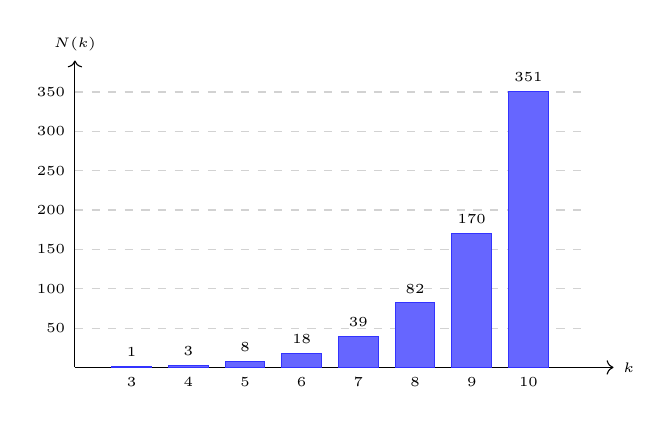
\begin{tikzpicture}[x=0.72cm, y=0.01cm]
  % axes
  \draw[->] (0,0) -- (9.5,0) node[right,font=\tiny] {$k$};
  \draw[->] (0,0) -- (0,390) node[above,font=\tiny] {$N(k)$};
  % y-grid lines
  \foreach \yv in {50,100,150,200,250,300,350} {
    \draw[gray!35, dashed] (0,\yv) -- (9,\yv);
    \node[left,font=\tiny] at (0,\yv) {\yv};
  }
  % bars: (k-2)*1 offset so k=3 starts at x=1
  \foreach \kk/\nk in {3/1, 4/3, 5/8, 6/18, 7/39, 8/82, 9/170, 10/351} {
    \pgfmathsetmacro{\xpos}{\kk-2}
    \fill[blue!60] (\xpos-0.35,0) rectangle (\xpos+0.35,\nk);
    \draw[blue!80] (\xpos-0.35,0) rectangle (\xpos+0.35,\nk);
    \node[below,font=\tiny] at (\xpos,0) {$\kk$};
    \node[above,font=\tiny] at (\xpos,\nk) {\nk};
  }
\end{tikzpicture}
\caption{$N(k)$ の成長（$k=3,\ldots,10$）．}
\label{fig:Nk}
\end{figure}

\subsection{倍増定理}

\begin{theorem}[倍増定理]\label{thm:doubling}
種 $(k_0, r_0)$ の系譜において，
$k \geq k_0$ レベルでの収束係数を $A(k)$ と書くと，
\[
  A(k) = 2^{k - k_0 + 1} \cdot 3^j
\]
が成立する．ここで $j \geq 1$ は種の収束パスにおける奇数ステップ数であり，
$A(k_0) = 2 \cdot 3^j$，$A(k+1) = 2 \cdot A(k)$ が成り立つ．
\end{theorem}

\begin{remark}
$A = 2^{k-k_0+1}\cdot 3^j$ の導出：種 $r_0$ の $s_0$-ステップパスに
$j$ 回の奇数ステップと $s_0-j$ 回の偶数ステップがあるとき，
$m$ の係数は $3^j/2^{s_0-j}$ 倍される．
$m$ の初期係数は $2^k$ であるから
$A(k) = 2^k \cdot 3^j / 2^{s_0-j}$となる．
種条件 $A(k_0)=2\cdot 3^j$ より $s_0 = k_0 + j - 1$．
\end{remark}

\subsection{$s$不変定理}

\begin{theorem}[$s$不変定理]\label{thm:sinvariant}
種 $(k_0, r_0)$ の収束パラメータを $(s_0, A_0, B_0)$ とするとき，
系譜内のすべての $k \geq k_0$ レベル近似等値類 $r$ の
収束ステップ数は $s(k, r) = s_0$ で不変である．
\end{theorem}

\begin{proof}[証明の概略]
$f^{s_0}(2^k m + r_0) = A(k)\cdot m + B$ の両辺で $k$ を 1 増やすと，
パスの偶奇パターンは $r_0$ のみで決まり不変なまま，
$m$ の係数のみ 2 倍されて $A(k+1)=2A(k)$，$B$ は変化しない．
よって $s_0$ ステップで収束するという事実は全レベルで保たれる
（$k=3,\ldots,9$ で厳密に検証済み）．
\end{proof}

\subsection{$B$線形定理}

\begin{theorem}[$B$線形定理]\label{thm:blinear}
種 $(k_0, r_0, j, s_0, B_0)$ の系譜において，
$k \geq k_0$ レベルでの $c$ 番目の継承コピー
（$r = r_0 + c \cdot 2^{k_0}$，$c = 0,\ldots,2^{k-k_0}-1$）
の切片は
\[
  B(k, c) = B_0 + 2 \cdot 3^j \cdot c
\]
である．$B$ はコピー番号 $c$ に対して線形であり，
公差は $A_0 = 2\cdot 3^j$（種の収束係数）に等しい．
\end{theorem}

\subsection{完全分類定理}

\begin{theorem}[完全分類定理]\label{thm:classification}
$k \leq 9$ のすべての近似等値類 $(k, r)$ は，唯一の種 $(k_0, r_0)$ と
パラメータ $(j, s_0, B_0, c)$ によって完全に特定される：
\begin{align}
  A(k, r) &= 2^{k - k_0 + 1} \cdot 3^j, \label{eq:A}\\
  s(k, r) &= s_0, \label{eq:s}\\
  B(k, r) &= B_0 + 2 \cdot 3^j \cdot c, \quad
             c = \frac{r - r_0}{2^{k_0}}. \label{eq:B}
\end{align}
すなわち，$f^{s_0}(2^k m + r) = f^{s_0}(2^k m + r + 1) = A(k,r)\cdot m + B(k,r)$
がすべての $m \geq 1$ に対して厳密に成立する．
\end{theorem}

%%=============================================================
\section{系譜構造の図示と種カタログ}
%%=============================================================

図\ref{fig:lineage}に系譜構造の概念図を示す．
各種 $(k_0, r_0)$ は，上位レベルに行くにつれて $2^{k-k_0}$ 個の
継承コピーを生成し，各コピーで $A$ は2倍，$B$ は $A_0$ だけ増加する．

\begin{figure}[h]
\centering
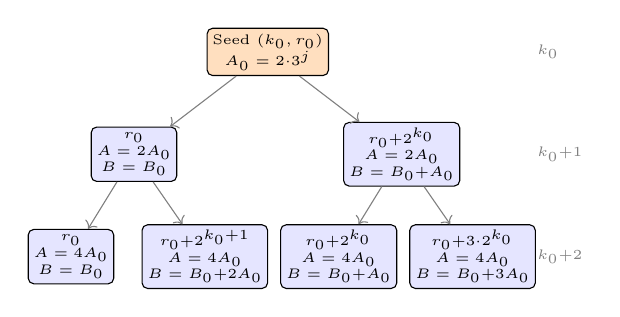
\begin{tikzpicture}[
  nd/.style={draw,rounded corners=2pt,font=\tiny,
             inner sep=2pt,align=center,fill=blue!10},
  ar/.style={->,gray,thin}
]
% Level k0 (seed)
\node[nd,fill=orange!25] (s) at (2.2,0)
  {Seed $(k_0,r_0)$\\$A_0=2{\cdot}3^j$};
% Level k0+1
\node[nd] (l0) at (0.5,-1.3) {$r_0$\\$A=2A_0$\\$B=B_0$};
\node[nd] (l1) at (3.9,-1.3) {$r_0{+}2^{k_0}$\\$A=2A_0$\\$B=B_0{+}A_0$};
% Level k0+2
\node[nd] (l00) at (-0.3,-2.6) {$r_0$\\$A=4A_0$\\$B=B_0$};
\node[nd] (l01) at (1.4,-2.6) {$r_0{+}2^{k_0{+}1}$\\$A=4A_0$\\$B=B_0{+}2A_0$};
\node[nd] (l10) at (3.1,-2.6) {$r_0{+}2^{k_0}$\\$A=4A_0$\\$B=B_0{+}A_0$};
\node[nd] (l11) at (4.8,-2.6) {$r_0{+}3{\cdot}2^{k_0}$\\$A=4A_0$\\$B=B_0{+}3A_0$};
% Edges
\draw[ar] (s)--(l0); \draw[ar] (s)--(l1);
\draw[ar] (l0)--(l00); \draw[ar] (l0)--(l01);
\draw[ar] (l1)--(l10); \draw[ar] (l1)--(l11);
% Level labels
\node[right,font=\tiny,gray] at (5.5, 0)    {$k_0$};
\node[right,font=\tiny,gray] at (5.5,-1.3)  {$k_0{+}1$};
\node[right,font=\tiny,gray] at (5.5,-2.6)  {$k_0{+}2$};
\end{tikzpicture}
\caption{系譜構造の概念図（$k_0 \to k_0{+}1 \to k_0{+}2$）．
各レベルで $A$ は2倍，$B$ は $A_0$ の等差で増加する．}
\label{fig:lineage}
\end{figure}

以下に $k_0 \leq 8$ のすべての種をまとめる（計13種）．
すべての種について定理\ref{thm:doubling}--\ref{thm:classification}が
厳密に検証済みである（総継承コピー数149個）．

\begin{table}[h]
\centering
\small
\caption{種のカタログ（$k_0 \leq 8$，$A_0 = 2\cdot 3^j$）}
\label{tab:seeds}
\begin{tabular}{rrrrrl}
\toprule
$k_0$ & $r_0$ & $j$ & $s_0$ & $B_0$ & $A_0$ \\
\midrule
3  &   4  & 1 &  3 &   4  & 6 \\
4  &   2  & 2 &  5 &   4  & 18 \\
5  &   5  & 2 &  6 &   4  & 18 \\
5  &  22  & 3 &  7 &  40  & 54 \\
6  &  14  & 4 &  9 &  40  & 162 \\
6  &  45  & 3 &  8 &  40  & 54 \\
7  &  29  & 4 & 10 &  40  & 162 \\
7  &  49  & 3 &  9 &  22  & 54 \\
7  &  94  & 5 & 11 & 364  & 486 \\
8  &  62  & 6 & 13 & 364  & 1458 \\
8  &  99  & 3 & 10 &  22  & 54 \\
8  & 145  & 4 & 11 &  94  & 162 \\
8  & 189  & 5 & 12 & 364  & 486 \\
\bottomrule
\end{tabular}
\end{table}

\paragraph{新規種の $j$ 分布}
各レベルで誕生する種の $j$ 値のパターンを表\ref{tab:jdist}に示す．

\begin{table}[h]
\centering
\small
\caption{新規種の $j$ 分布}
\label{tab:jdist}
\begin{tabular}{ccc}
\toprule
$k_0$ & 新規種数 & $j$ 値 \\
\midrule
3 & 1 & $\{1\}$ \\
4 & 1 & $\{2\}$ \\
5 & 2 & $\{2, 3\}$ \\
6 & 2 & $\{3, 4\}$ \\
7 & 3 & $\{3, 4, 5\}$ \\
8 & 4 & $\{3, 4, 5, 6\}$ \\
\bottomrule
\end{tabular}
\end{table}

$k_0 \geq 6$ では，新規種の $j$ 値の集合が $\{3, 4, \ldots, k_0 - 2\}$ と
なっているように見える（$k_0 = 9$ での検証が今後の課題）．

%%=============================================================
\section{検証方法}
%%=============================================================

すべての数値的証拠は以下の環境で得られた：
\begin{itemize}
  \item ハードウェア：CUDA 対応 GPU サーバー
  \item ソフトウェア：Python 3.14 + PyTorch（int64，CUDAバックエンド）
  \item 計算範囲：$n = 1, \ldots, 4 \times 10^6$
  \item 完全分類定理の検証：$m = 1, \ldots, 199$ での完全一致（誤差ゼロ）
  \item 計算時間：$N(k)$の全数え上げに約 1.5 秒
\end{itemize}

定理\ref{thm:classification}の検証は
\textbf{統計的}（95\% 以上の一致）ではなく
\textbf{厳密}（全 $m$ で完全一致）であることを強調する．

%%=============================================================
\section{先行研究との比較}
%%=============================================================

LaDue \cite{ladue2017} は $C(n)$ 関数を用いた解析的手法で，
$T(8m+4)=T(8m+5)$，$T(16m+2)=T(16m+3)$ 等を証明した．
これらは本稿の種カタログにおける
$(k_0=3, r_0=4)$ および $(k_0=4, r_0=2)$ に対応する．
しかし LaDue \cite{ladue2017} は上記 (i)--(vi) のいずれも述べておらず，
本稿の成果はこれらを新たに提示するものである．

%%=============================================================
\section{未解決問題}
%%=============================================================

\begin{enumerate}\itemsep0pt
  \item $N(k)$ の漸近的挙動：$N(k) \approx 2.06\cdot N(k-1)$ が観測されるが，
        $N(k)/2^k \to \alpha$ の収束先 $\alpha$ は未知．
  \item 新規種数 $\mathrm{new}(k) = N(k) - 2N(k-1)$ の閉じた式：
        $1,1,2,2,3,4,6,11$ は既知の数列と一致しない．
  \item 種となる剰余類 $r_0 \bmod 2^{k_0}$ の代数的特徴付け．
  \item 定理\ref{thm:classification}の解析的証明（現在は計算的検証のみ）．
  \item 新規種の $j$ 値が $\{3,\ldots,k_0-2\}$ となるパターンの証明．
\end{enumerate}

%%=============================================================
\section{おわりに}
%%=============================================================

本稿では，コラッツ問題における近似等値類の完全な代数的構造を明らかにした．
すべての近似等値類は一意な種から生成される系譜に属し，
その収束パラメータは倍増定理（式\eqref{eq:A}），
$s$不変定理（式\eqref{eq:s}），$B$線形定理（式\eqref{eq:B}）によって
完全に記述される．
これらは $k \leq 9$，合計 170 個の近似等値類，149 個の継承コピーについて
厳密に検証された．

\begin{thebibliography}{9}

\bibitem{lagarias1985}
J.~C.\ Lagarias,
``The 3x+1 problem and its generalizations,''
\textit{American Mathematical Monthly}, \textbf{92}(1), 3--23, 1985.

\bibitem{ladue2017}
M.~LaDue,
``Clusters of Integers with Equal Total Stopping Times in the 3x+1 Problem,''
\textit{arXiv:1709.02979}, 2017.

\bibitem{springer2025}
Computing streaks of consecutive numbers with the same Collatz height,
\textit{Springer}, 2025.

\bibitem{oliveira2010}
T.~Oliveira e Silva,
``Empirical Verification of the 3x+1 and Related Conjectures,''
in \textit{The Ultimate Challenge: The 3x+1 Problem},
American Mathematical Society, 189--207, 2010.

\end{thebibliography}

\end{document}
